\documentclass[10pt,a4paper,UTF8,fontset=windows]{ctexart}

\usepackage[a4paper,left=1.55cm,right=1.55cm,top=1.55cm,bottom=1.65cm]{geometry}
\usepackage{amsmath,amssymb}
\usepackage{array,booktabs,multirow,tabularx}
\usepackage{graphicx}
\usepackage{xcolor}
\usepackage{enumitem}
\usepackage{caption}
\usepackage{float}
\usepackage{hyperref}
\usepackage{url}
\usepackage{listings}
\usepackage{fancyhdr}
\usepackage{microtype}

\graphicspath{{assets/}}
\definecolor{accent}{HTML}{17365D}
\definecolor{lightblue}{HTML}{EAF3F8}
\definecolor{lightgray}{HTML}{F4F6F8}
\definecolor{darkgray}{HTML}{4B5563}
\hypersetup{
  colorlinks=true,
  linkcolor=accent,
  urlcolor=accent,
  citecolor=accent,
  pdfauthor={陈家龙},
  pdftitle={计算机视觉 HW3 实验报告}
}
\urlstyle{same}
\captionsetup{font=small,labelfont=bf}
\setlist{nosep,leftmargin=1.5em}
\setlength{\columnsep}{0.72cm}
\setlength{\parindent}{2em}
\setlength{\parskip}{0.15em}
\renewcommand{\arraystretch}{1.22}
\newcolumntype{Y}{>{\raggedright\arraybackslash}X}
\newcommand{\code}[1]{\texttt{\small #1}}
\newcommand{\taskoneweights}{https://github.com/Loong-C/FDU-Computer-Vision/releases/download/hw3-task1-weights/cv-hw3-task1-best-weights.tar.gz}
\newcommand{\taskonevideo}{https://github.com/Loong-C/FDU-Computer-Vision/releases/download/hw3-task1-weights/task1-walkthrough.mp4}
\newcommand{\tasktwocode}{https://github.com/Loong-C/FDU-Computer-Vision/tree/main/hw3/task2}
\newcommand{\tasktworelease}{https://github.com/Loong-C/FDU-Computer-Vision/releases/tag/hw3-task2-formal-partial-v1}
\newcommand{\tasktwobweights}{https://github.com/Loong-C/FDU-Computer-Vision/releases/download/hw3-task2-formal-partial-v1/hw3-task2-act-b-only-best.pt}
\newcommand{\tasktwoabcweights}{https://github.com/Loong-C/FDU-Computer-Vision/releases/download/hw3-task2-formal-partial-v1/hw3-task2-act-abc-joint-best.pt}
\newcommand{\clouddrive}{https://drive.google.com/drive/folders/1v9oc1uTbZS31SaDJaT7sYV8m5dutMo1y?usp=drive_link}

\pagestyle{fancy}
\fancyhf{}
\fancyhead[L]{\small 计算机视觉 HW3}
\fancyhead[R]{\small 陈家龙（24300980041）}
\fancyfoot[C]{\small \thepage}
\renewcommand{\headrulewidth}{0.35pt}
\renewcommand{\footrulewidth}{0pt}

\lstset{
  basicstyle=\ttfamily\scriptsize,
  breaklines=true,
  columns=fullflexible,
  frame=single,
  backgroundcolor=\color{lightgray},
  rulecolor=\color{gray!40},
  xleftmargin=0.3em,
  xrightmargin=0.3em
}

\begin{document}
\sloppy

\begin{titlepage}
  \thispagestyle{empty}
  \centering
  \vspace*{1.4cm}
  {\Large 复旦大学计算机视觉课程期末作业\par}
  \vspace{0.65cm}
  {\fontsize{24}{31}\selectfont\bfseries 计算机视觉 HW3 实验报告\par}
  \vspace{0.35cm}
  {\Large\bfseries 多源 3D 场景融合与 ACT 跨环境泛化\par}
  \vspace{1.05cm}

  \begin{tabularx}{0.88\textwidth}{>{\bfseries}p{3.1cm}Y}
    \toprule
    项目 & 内容 \\
    \midrule
    姓名 & 陈家龙 \\
    学号 & 24300980041 \\
    组队情况 & 单人完成 \\
    具体分工 & 独立完成 \\
    报告日期 & 2026 年 6 月 7 日 \\
    \bottomrule
  \end{tabularx}

  \vspace{0.85cm}
  {\large\bfseries 提交链接\par}
  \vspace{0.25cm}
  \begin{tabularx}{0.94\textwidth}{>{\bfseries}p{3.0cm}Y}
    \toprule
    项目 & 可公开访问地址 \\
    \midrule
    题目一代码仓库 &
    \href{https://github.com/Loong-C/FDU-Computer-Vision/tree/main/hw3/task1}{github.com/Loong-C/FDU-Computer-Vision（main/hw3/task1）} \\
    题目一模型权重 &
    \href{\taskoneweights}{GitHub Release：cv-hw3-task1-best-weights.tar.gz} \\
    题目一漫游视频 &
    \href{\taskonevideo}{GitHub Release：task1-walkthrough.mp4} \\
    题目二代码仓库 &
    \href{\tasktwocode}{github.com/Loong-C/FDU-Computer-Vision（main/hw3/task2）} \\
    题目二模型权重 &
    \href{\tasktworelease}{FDU GitHub Release：hw3-task2-formal-partial-v1} \\
    题目二 SwanLab &
    \href{https://swanlab.cn/@Linkukai/hw3-calvin-act}{swanlab.cn/@Linkukai/hw3-calvin-act} \\
    网盘镜像 &
    \href{\clouddrive}{模型、视频与报告镜像文件夹} \\
    \bottomrule
  \end{tabularx}

  \vfill
  \begin{minipage}{0.90\textwidth}
    \small
    \textbf{提交说明。}
    题目一包含 2DGS、AIGC 与 Blender 融合流程；题目二包含资源约束下基于官方
    CALVIN 帧的 ACT 对比实验。训练曲线由 SwanLab 记录导出。模型权重和视频提供
    公开下载地址；题目一资产包、漫游视频和题目二权重均提供 FDU GitHub Release，
    Google Drive 继续作为镜像目录。
  \end{minipage}
  \vspace{0.7cm}
\end{titlepage}

\twocolumn

\begin{abstract}
本作业包含两个相互独立但都强调完整实验链路的视觉任务。题目一从真实采集、文本生成和
单图生成三种来源构建 3D 资产，使用 2D Gaussian Splatting（2DGS）重建真实物体与
Mip-NeRF 360 背景，并将异构表示统一为 Mesh 后在 Blender 中完成融合渲染。题目二使用
LeRobot 中的 ACT 策略，在 CALVIN 环境 B 与混合环境 A+B+C 上分别训练模型，再在未见过的
环境 D 上比较离线零样本动作误差，并补充 CALVIN simulator rollout 成功率。实验表明：
多视角重建在几何可靠性上最强，文本到 3D 输入成本
最低，单图到 3D 则在真实外观保持与采集成本之间折中；ACT 的多环境训练虽然提高了同分布
验证损失，却使环境 D 的 first-action MAE 和 chunk-action MAE 分别下降 17.0\% 和 11.7\%。
两个策略在 3 条环境 D simulator 五任务序列上的 SR@1--SR@5 均为 0，说明离线动作误差与
长时闭环成功率反映的是不同层次的泛化能力。
\end{abstract}

\section{作业目标与实验组织}

课程作业包含 3D 视觉场景融合与具身策略泛化两道题。题目一需要处理四类来源不同、原生表示
不同的资产，并将其组合为可渲染的统一场景。题目二保持 ACT 网络架构和超参数一致，仅改变训练
环境分布，用于观察视觉分布偏移下的零样本行为。

所有长时间实验均由可追踪脚本启动。题目一将 2DGS TensorBoard 标量与 AIGC 训练指标导入
SwanLab 本地运行；题目二在 SwanLab 中记录 Action L1、KL、验证损失、环境 D 动作误差和
simulator rollout 成功率，同时保留 CSV/JSON 备份。报告中的曲线均由记录指标生成。

\section{题目一：2DGS 与 AIGC 多源资产融合}

\subsection{要求拆解与数据准备}

题目一要求准备三个独立 3D 物体，并将它们放入同一真实背景：物体 A 必须由手机多视角拍摄、
COLMAP 位姿估计和 2DGS 重建得到；物体 B 必须仅由文本 Prompt 驱动 threestudio 与 SDS
优化得到；物体 C 必须由一张真实物体照片经过去背景后输入 Magic123；背景场景则来自公开 3D
数据集并使用 2DGS 重建。本实验选择 Mip-NeRF 360 的 \code{counter} 场景作为统一环境。

\begin{table}[H]
\centering
\caption{题目一数据与预处理。}
\label{tab:task1-data}
\resizebox{\columnwidth}{!}{
\begin{tabular}{p{1.25cm}p{2.5cm}p{3.45cm}}
\toprule
资产 & 输入规模 & 准备过程 \\
\midrule
物体 A & 手机照片 63 张，其中注册 34 张 & COLMAP 特征匹配、稀疏重建、去畸变 \\
物体 B & 文本 Prompt 1 条 & 固定产品描述，直接驱动 SDS 优化 \\
物体 C & 手机实拍图 1 张，$1448\times1086$ & 棋盘格背景去除、RGBA 前景、MiDaS 深度 \\
背景 & \code{counter} 多视角图 240 张 & 选择性下载开源场景，复用相机参数 \\
\bottomrule
\end{tabular}}
\end{table}

物体 A 的 COLMAP 稀疏模型最终包含 1527 个稀疏点和 5203 次观测，平均轨迹长度为
3.407335，平均每张图像包含 153.029412 次观测，平均重投影误差为 1.192686 像素。
这说明筛选后的 34 个视角具有足够重叠，可用于后续显式表面优化。物体 C 采用药盒作为输入：
先得到干净的 alpha 前景，再构建 Magic123 所需的 RGBA 与深度先验。

\begin{figure*}[t]
  \centering
  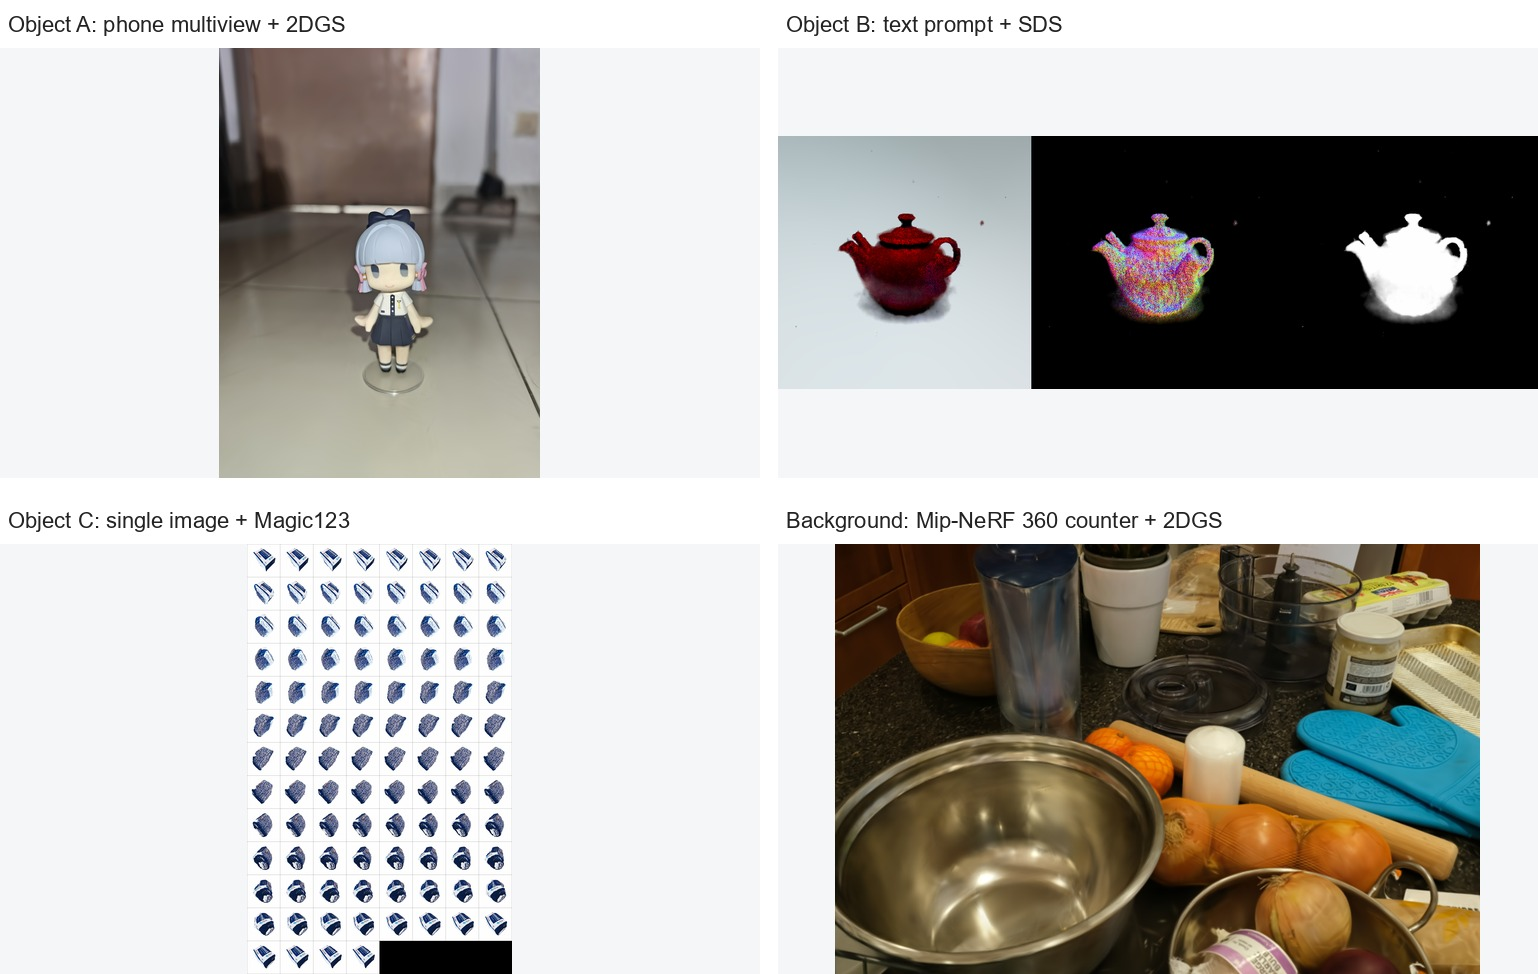
\includegraphics[width=0.94\textwidth]{asset_preview_montage.jpg}
  \caption{题目一的四类输入与阶段性产物。物体 A 来自真实手机多视角，物体 B 由文本生成，
  物体 C 来自单图，背景为 Mip-NeRF 360 \code{counter} 场景。}
  \label{fig:task1-assets}
\end{figure*}

\subsection{真实物体与背景：COLMAP + 2DGS}

COLMAP 首先从多视角图像恢复相机内外参与稀疏点云。之后使用 2DGS 将场景表示为一组具有中心、
尺度、旋转、颜色、不透明度和球谐系数的二维高斯面片。与体积型 3D Gaussian Splatting 相比，
2DGS 更强调表面对齐，因此更适合在重建后提取网格。像素重建损失使用 L1 与 DSSIM 组合：
\begin{equation}
  \mathcal{L}_{\text{rgb}}
  = (1-\lambda_{\text{dssim}})\mathcal{L}_{1}
  + \lambda_{\text{dssim}}(1-\text{SSIM}).
\end{equation}
正式配置中 $\lambda_{\text{dssim}}=0.2$。在第 7000 步后，额外启用
$\lambda_{\text{normal}}=0.05$ 的法线一致性正则；失真正则权重设为 0。物体 A 使用原始分辨率，
背景 \code{counter} 使用半分辨率，两者均训练 30000 步。

\subsection{文本到 3D：threestudio DreamFusion SDS}

物体 B 的 Prompt 为：
\begin{quote}\small
\textit{A studio product photo of a small red ceramic teapot with a round body,
short spout, and curved handle.}
\end{quote}
threestudio 的 DreamFusion 路线将待优化物体表示为隐式体场，从随机相机渲染图像，并使用
Stable Diffusion 1.5 提供 SDS 梯度。训练过程中无需真实 3D 监督，当前渲染在扩散模型的
噪声预测空间内逐渐接近文本条件。简化后的梯度可写为
\begin{equation}
  \nabla_{\theta}\mathcal{L}_{\text{SDS}}
  \approx
  \mathbb{E}_{t,\epsilon}
  \left[
  w(t)(\hat{\epsilon}_{\phi}(x_t;y,t)-\epsilon)
  \frac{\partial x}{\partial\theta}
  \right].
\end{equation}
本实验训练 10000 步，随机视角分辨率为 $64\times64$，使用 Adam 优化器。正式导出的
OBJ 包含 28180 个顶点和 56536 个三角面。

\subsection{单图到 3D：Magic123}

物体 C 的单张图像只能约束可见表面，因此恢复不可见侧面时必须依赖生成先验。本实验先移除
棋盘格背景，通过 alpha 前景避免背景纹理进入重建，再使用 MiDaS 估计深度。Magic123 的 coarse
阶段同时使用 Stable Diffusion 1.5 的二维语义先验与 Zero123 的新视角先验优化 NeRF；fine
阶段从 coarse 检查点初始化 DMTet，并输出带纹理 Mesh。受本机 8 GB GPU 与主存约束影响，
本地正式实验采用 coarse 500 步和 fine 500 步；Magic123 参考预算为每阶段 5000 步。最终 OBJ
包含 22860 个顶点和 45730 个三角面。

\subsection{异构表示统一与场景融合}

四类资产采用不同的原生形式：2DGS 是显式高斯面片，DreamFusion 与 Magic123 在优化阶段分别
使用隐式体场和 NeRF/DMTet。直接在高斯参数层拼接需要为每种 AIGC 资产重新设计采样、初始化和
外观拟合流程，且不利于稳定控制遮挡和尺度。本实验选择\textbf{带颜色或纹理的 Mesh 作为交换表示}：
物体 A 与背景从 2DGS 通过有界 TSDF 表面提取获得 PLY；物体 B 与物体 C 从各自生成框架导出 OBJ。

\begin{figure*}[t]
  \centering
  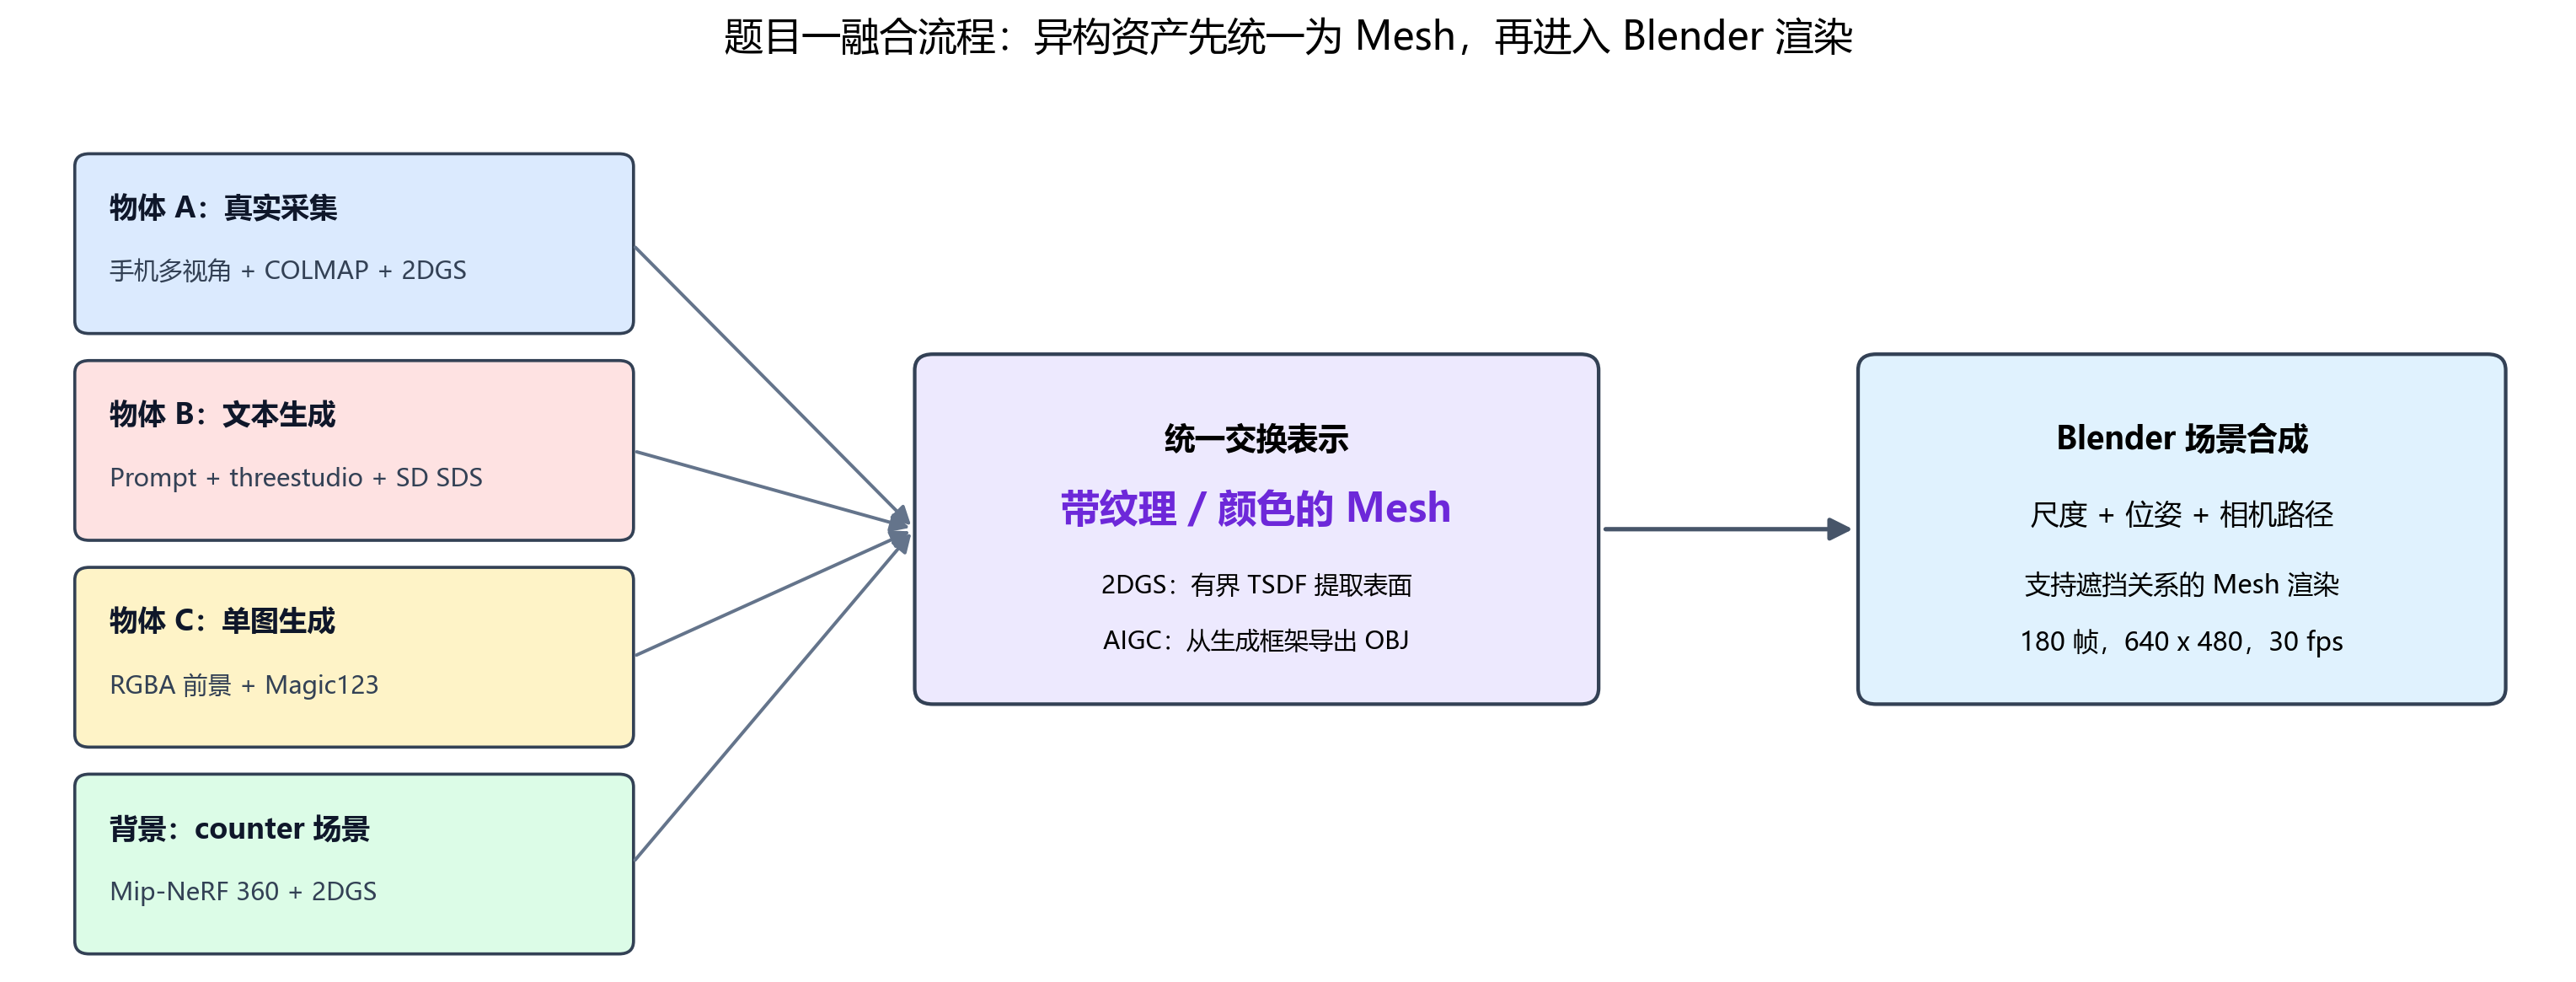
\includegraphics[width=0.98\textwidth]{task1_fusion_pipeline.png}
  \caption{题目一统一表示与融合流程。不同来源先转换为 Mesh，再在 Blender 中完成尺度、位姿、
  光照与相机轨迹设置。}
  \label{fig:fusion-pipeline}
\end{figure*}

Blender 场景中，背景保持原尺度；物体 A、B、C 分别放置在
$(-0.620,1.750,-0.254)$、$(-0.013,1.995,-0.306)$ 和
$(0.719,2.012,-0.315)$，尺度分别设为 0.10、0.40 和 0.60。相机路径从
\code{counter} 的 COLMAP 位姿导出，最终渲染 180 帧、$640\times480$、30 fps 的多视角漫游视频。
实现过程分为表示转换和场景编排两个步骤。前一步保证资产可互操作，后一步用于统一控制遮挡关系、
光照和相机运动。

\subsection{题目一实验设置}

正式实验的设置集中在表~\ref{tab:task1-hyper} 中。2DGS 部分沿用官方优化参数，并分别记录
物体 A 与背景场景的验证指标；DreamFusion 与 Magic123 记录实际迭代数、渲染分辨率、
优化器和 guidance 权重。后续的验证曲线、三视图比较和耗时统计均对应这一组设置。

\begin{table*}[t]
\centering
\caption{题目一主要超参数。2DGS 使用官方参数组；Magic123 的本地正式预算根据硬件约束调整。}
\label{tab:task1-hyper}
\small
\begin{tabularx}{0.98\textwidth}{p{2.45cm}p{1.8cm}p{2.1cm}Y Y}
\toprule
阶段 & 迭代 / 分辨率 & 优化器 & 关键参数 & 损失与监控指标 \\
\midrule
物体 A 2DGS &
30000 / 原始尺寸 &
官方 2DGS Adam &
位置 LR $1.6{\times}10^{-4}\rightarrow1.6{\times}10^{-6}$；
特征 LR 0.0025；不透明度 LR 0.05；尺度 LR 0.005；旋转 LR 0.001 &
L1 + DSSIM；法线正则 0.05；PSNR、验证 L1、高斯点数 \\
背景 \code{counter} 2DGS &
30000 / half &
同上 &
与物体 A 相同；半分辨率降低显存与时间成本 &
L1 + DSSIM；法线正则 0.05；PSNR、验证 L1、高斯点数 \\
物体 B DreamFusion &
10000 / $64\times64$ &
Adam &
batch size 1；geometry LR 0.01；background LR 0.001；
guidance scale 100；mixed precision &
SDS 1.0；sparsity 1.0；方向正则调度；SDS 曲线 \\
物体 C Magic123 coarse &
500 / $128\times128$ &
Adam &
SD / Zero123 guidance scale 100 / 5；
\code{lambda\_guidance=[1.0, 40]} &
总损失与两个 guidance 分量 \\
物体 C Magic123 fine &
500 / DMTet &
Adam &
coarse checkpoint 初始化；
\code{lambda\_guidance=[1e-3, 0.01]} &
总损失、guidance 分量、最终纹理 Mesh \\
\bottomrule
\end{tabularx}
\end{table*}

\subsection{题目一结果与分析}

\begin{table}[H]
\centering
\caption{2DGS 验证指标。}
\label{tab:2dgs-results}
\resizebox{\columnwidth}{!}{
\begin{tabular}{lrrrr}
\toprule
资产 & 迭代 & PSNR (dB) & 验证 L1 & 高斯点数 \\
\midrule
物体 A & 7000 & 31.8275 & 0.015616 & 149488 \\
物体 A & 30000 & 33.5198 & 0.011289 & 212465 \\
\code{counter} & 7000 & 28.0689 & 0.021551 & 482345 \\
\code{counter} & 30000 & 29.9138 & 0.016986 & 533358 \\
\bottomrule
\end{tabular}}
\end{table}

\begin{figure*}[t]
  \centering
  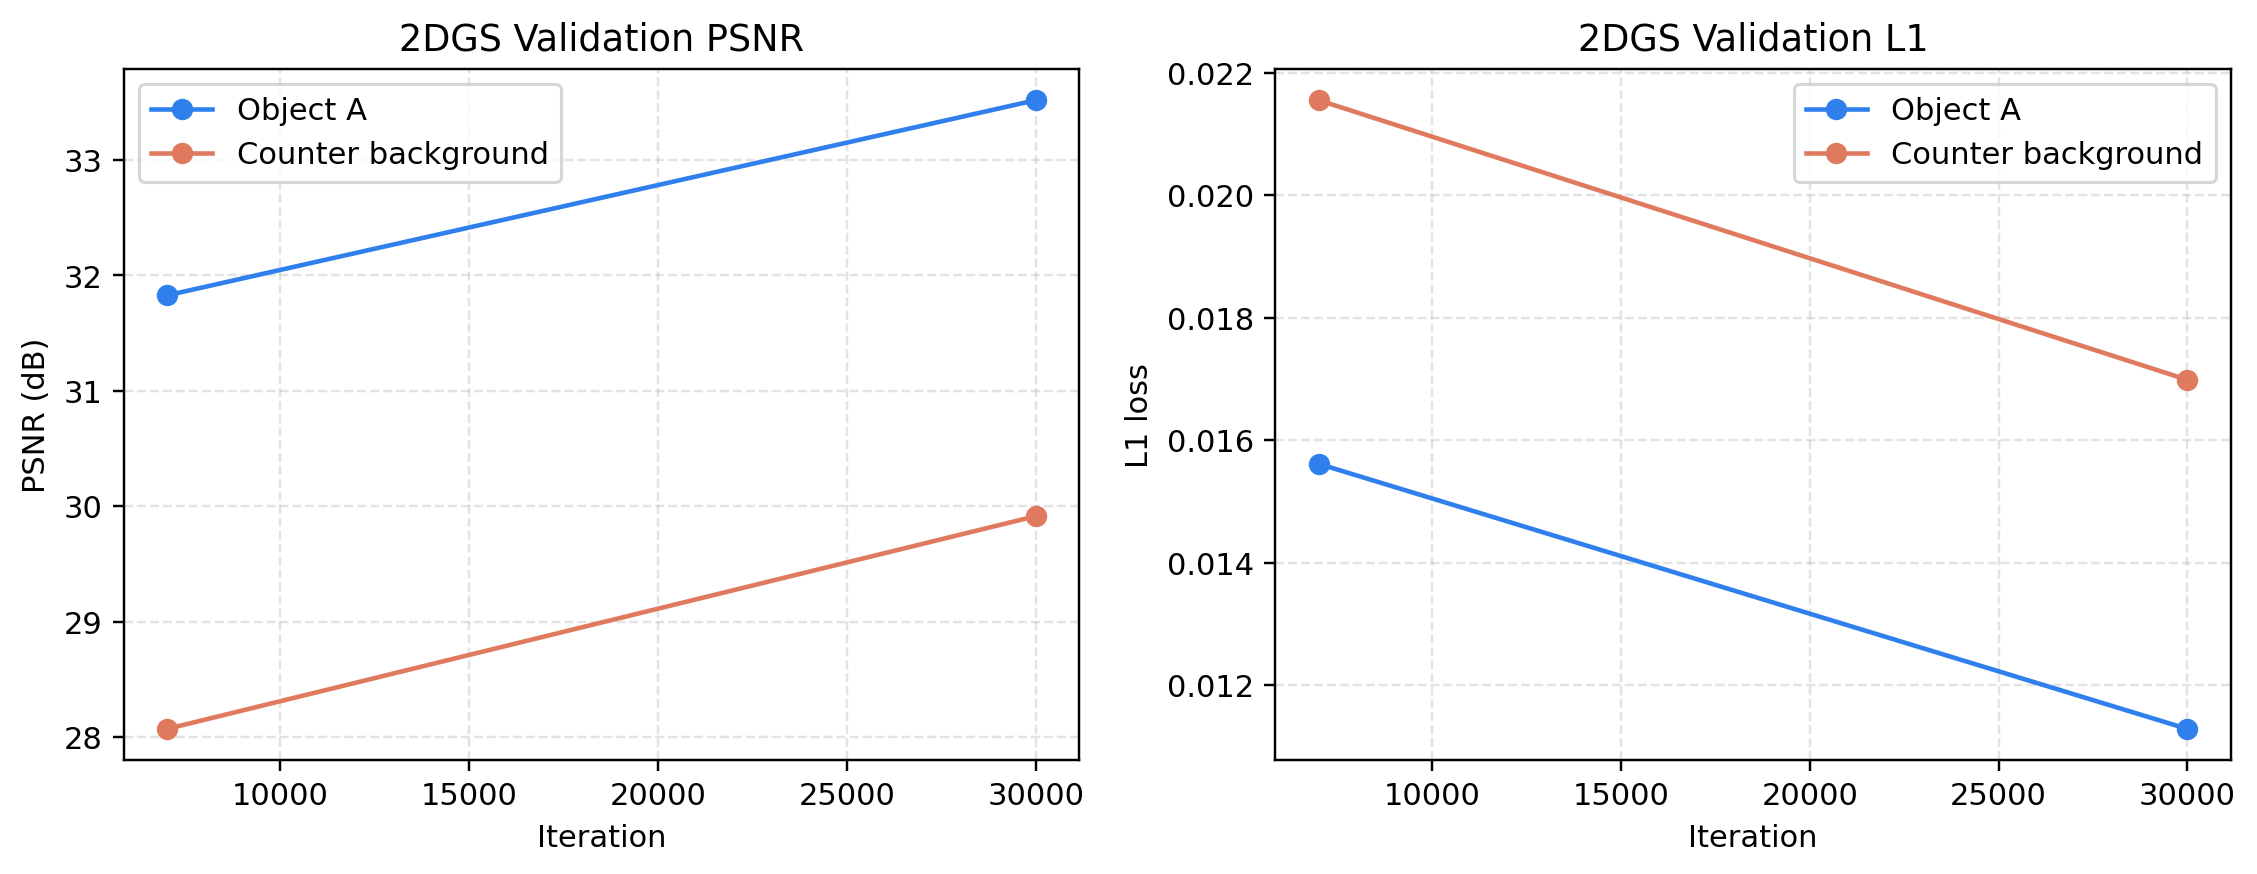
\includegraphics[width=0.94\textwidth]{2dgs_validation_metrics.png}
  \caption{由 SwanLab 记录指标导出的 2DGS 验证曲线。物体 A 与背景在 30000 步时均优于
  7000 步检查点：PSNR 上升且 L1 下降。}
  \label{fig:2dgs-metrics}
\end{figure*}

物体 A 从第 7000 步到第 30000 步的 PSNR 提升 1.6923 dB，验证 L1 下降约 27.7\%；
背景 PSNR 提升 1.8449 dB，验证 L1 下降约 21.2\%。背景的点数明显更多，因为厨房台面包含
更多遮挡、反光与细粒度结构。高斯点数增长与验证指标改善同时出现，表明增密过程补充了有效的
表面细节。

\begin{figure*}[t]
  \centering
  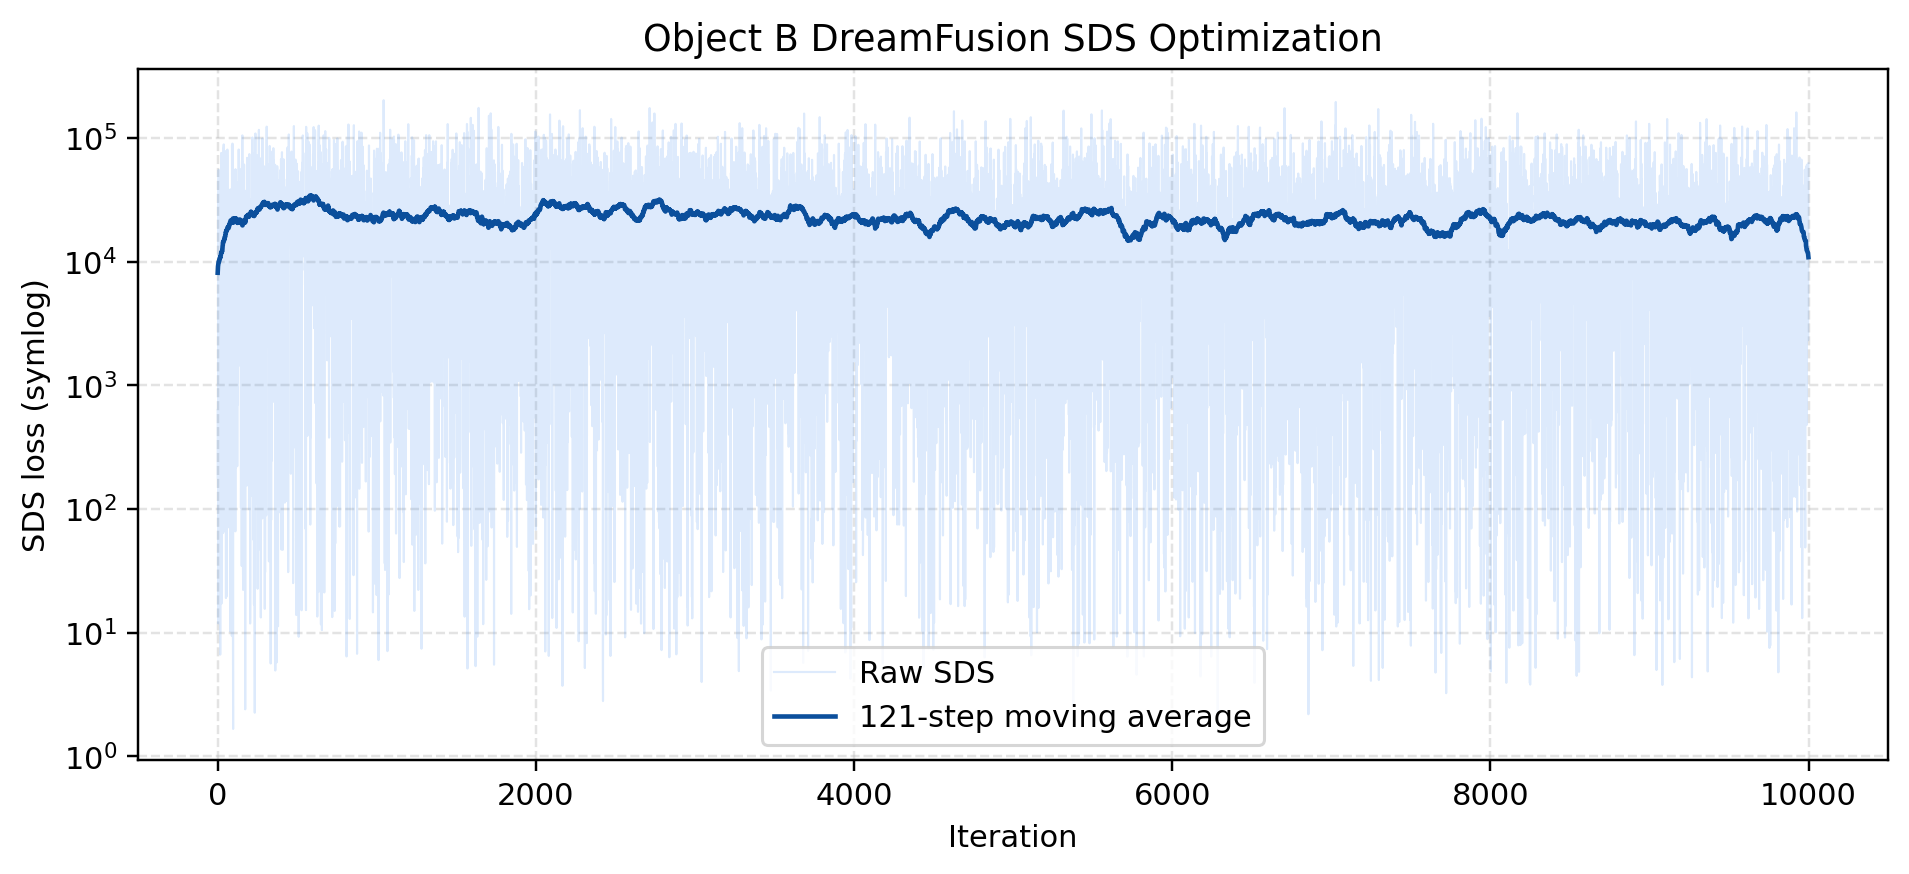
\includegraphics[width=0.48\textwidth]{object_b_sds_curve.png}
  \hfill
  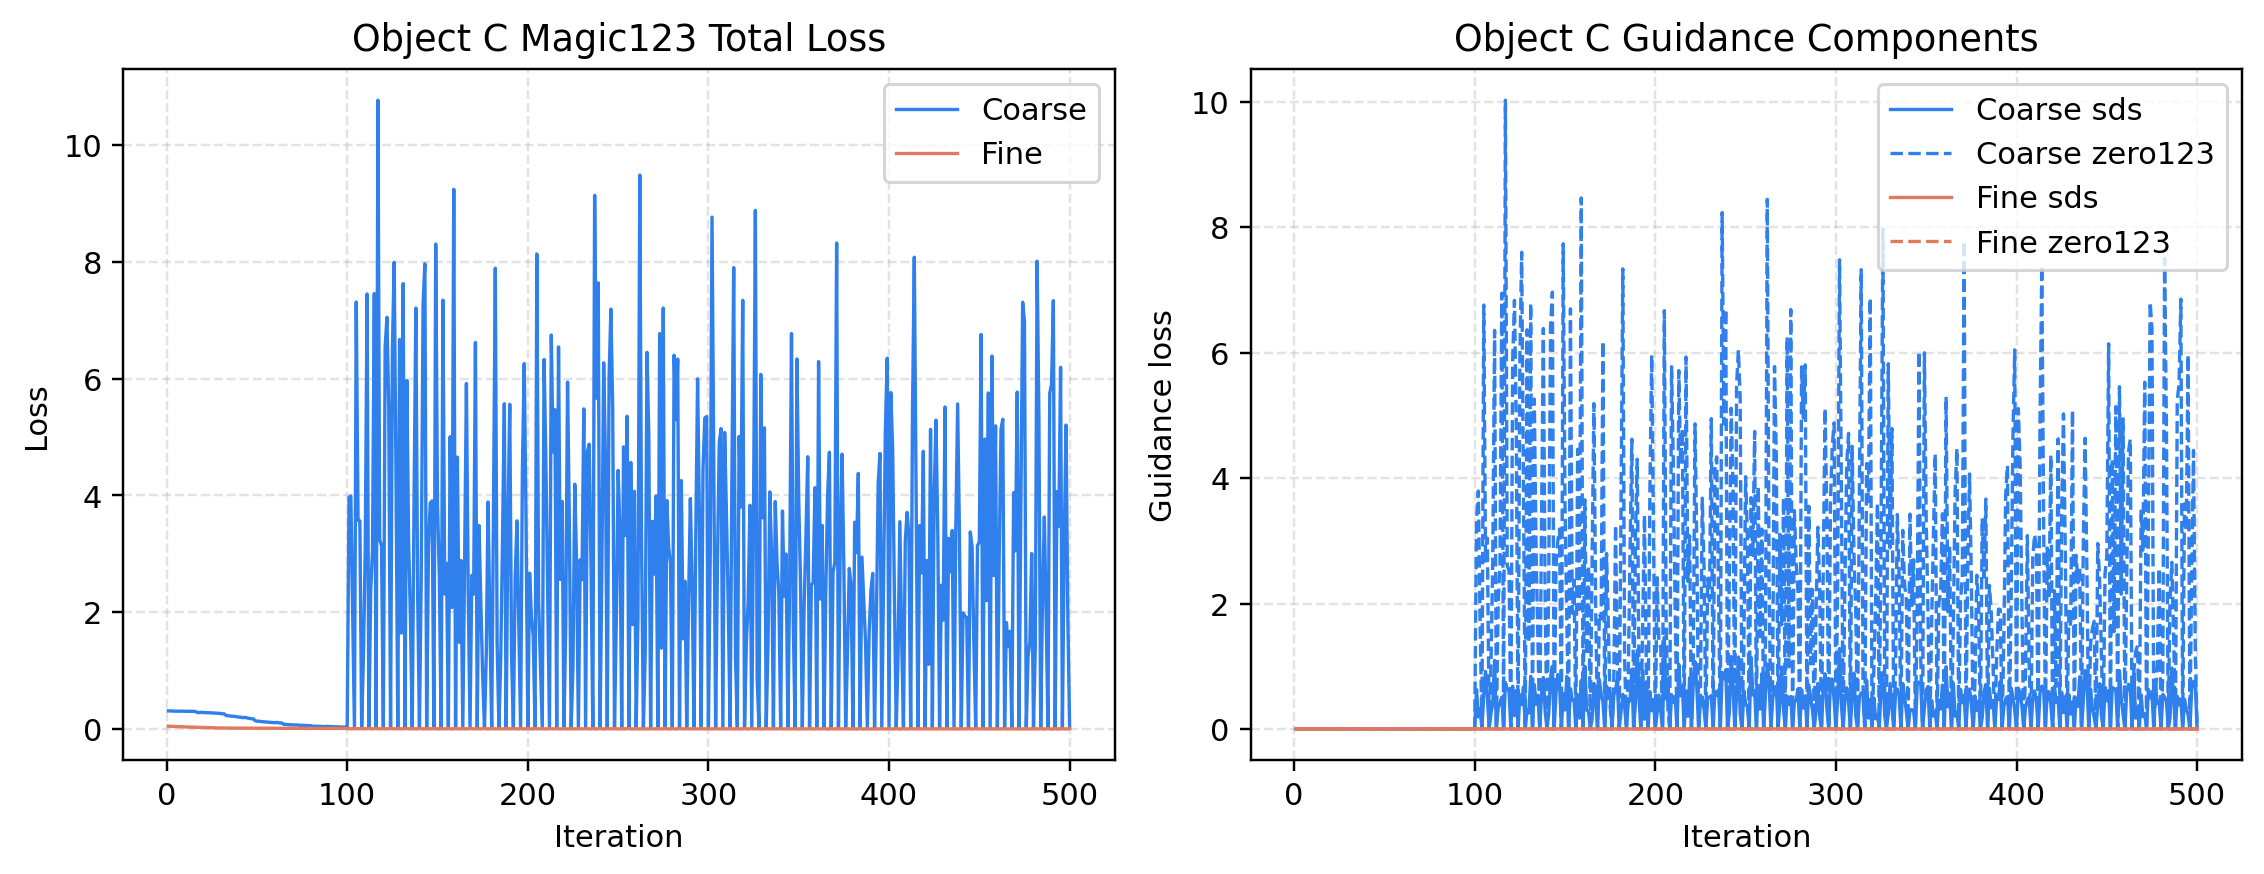
\includegraphics[width=0.48\textwidth]{object_c_magic123_losses.png}
  \caption{由 SwanLab 记录指标导出的 AIGC 优化曲线。左：物体 B 的 SDS 原始值与移动平均；
  右：物体 C 的 Magic123 总损失与 guidance 分量。生成式优化具有显著随机波动，因此曲线
  主要用于观察训练稳定性与阶段完成情况。}
  \label{fig:aigc-curves}
\end{figure*}

物体 B 的 SDS 曲线存在高频波动，这是随机相机、随机噪声步与扩散先验共同作用的结果。最终预览
能够辨认红色陶瓷茶壶的壶盖、短壶嘴、圆形壶身和弯曲把手，说明文本语义已经转化为可用类别形状；
但局部几何缺少真实观测作为验证依据。物体 C 的正面受到输入照片约束，药盒外观得以保留；侧面
和背面主要依靠生成先验补全，其几何真实性相对有限。

\subsubsection{代表性三视图与还原质量分析}

图~\ref{fig:task1-triviews} 从三个方向展示三种方法的输出。物体 A 使用 2DGS 导出的
\code{fuse\_post.ply}，裁剪出手办主体后进行正交渲染。原始 TSDF Mesh 还包含少量邻近地面残片，
裁剪时保留了贴近主体的表面提取结果，便于观察真实的网格质量。物体 B 选取 DreamFusion 环绕序列
\code{0/30/60}；物体 C 选取 Magic123 Lambertian 环绕序列 \code{0000/0025/0050}。
这些视图用于比较外观、轮廓和跨视角稳定性，不用于精确尺寸测量。

\begin{figure*}[t]
  \centering
  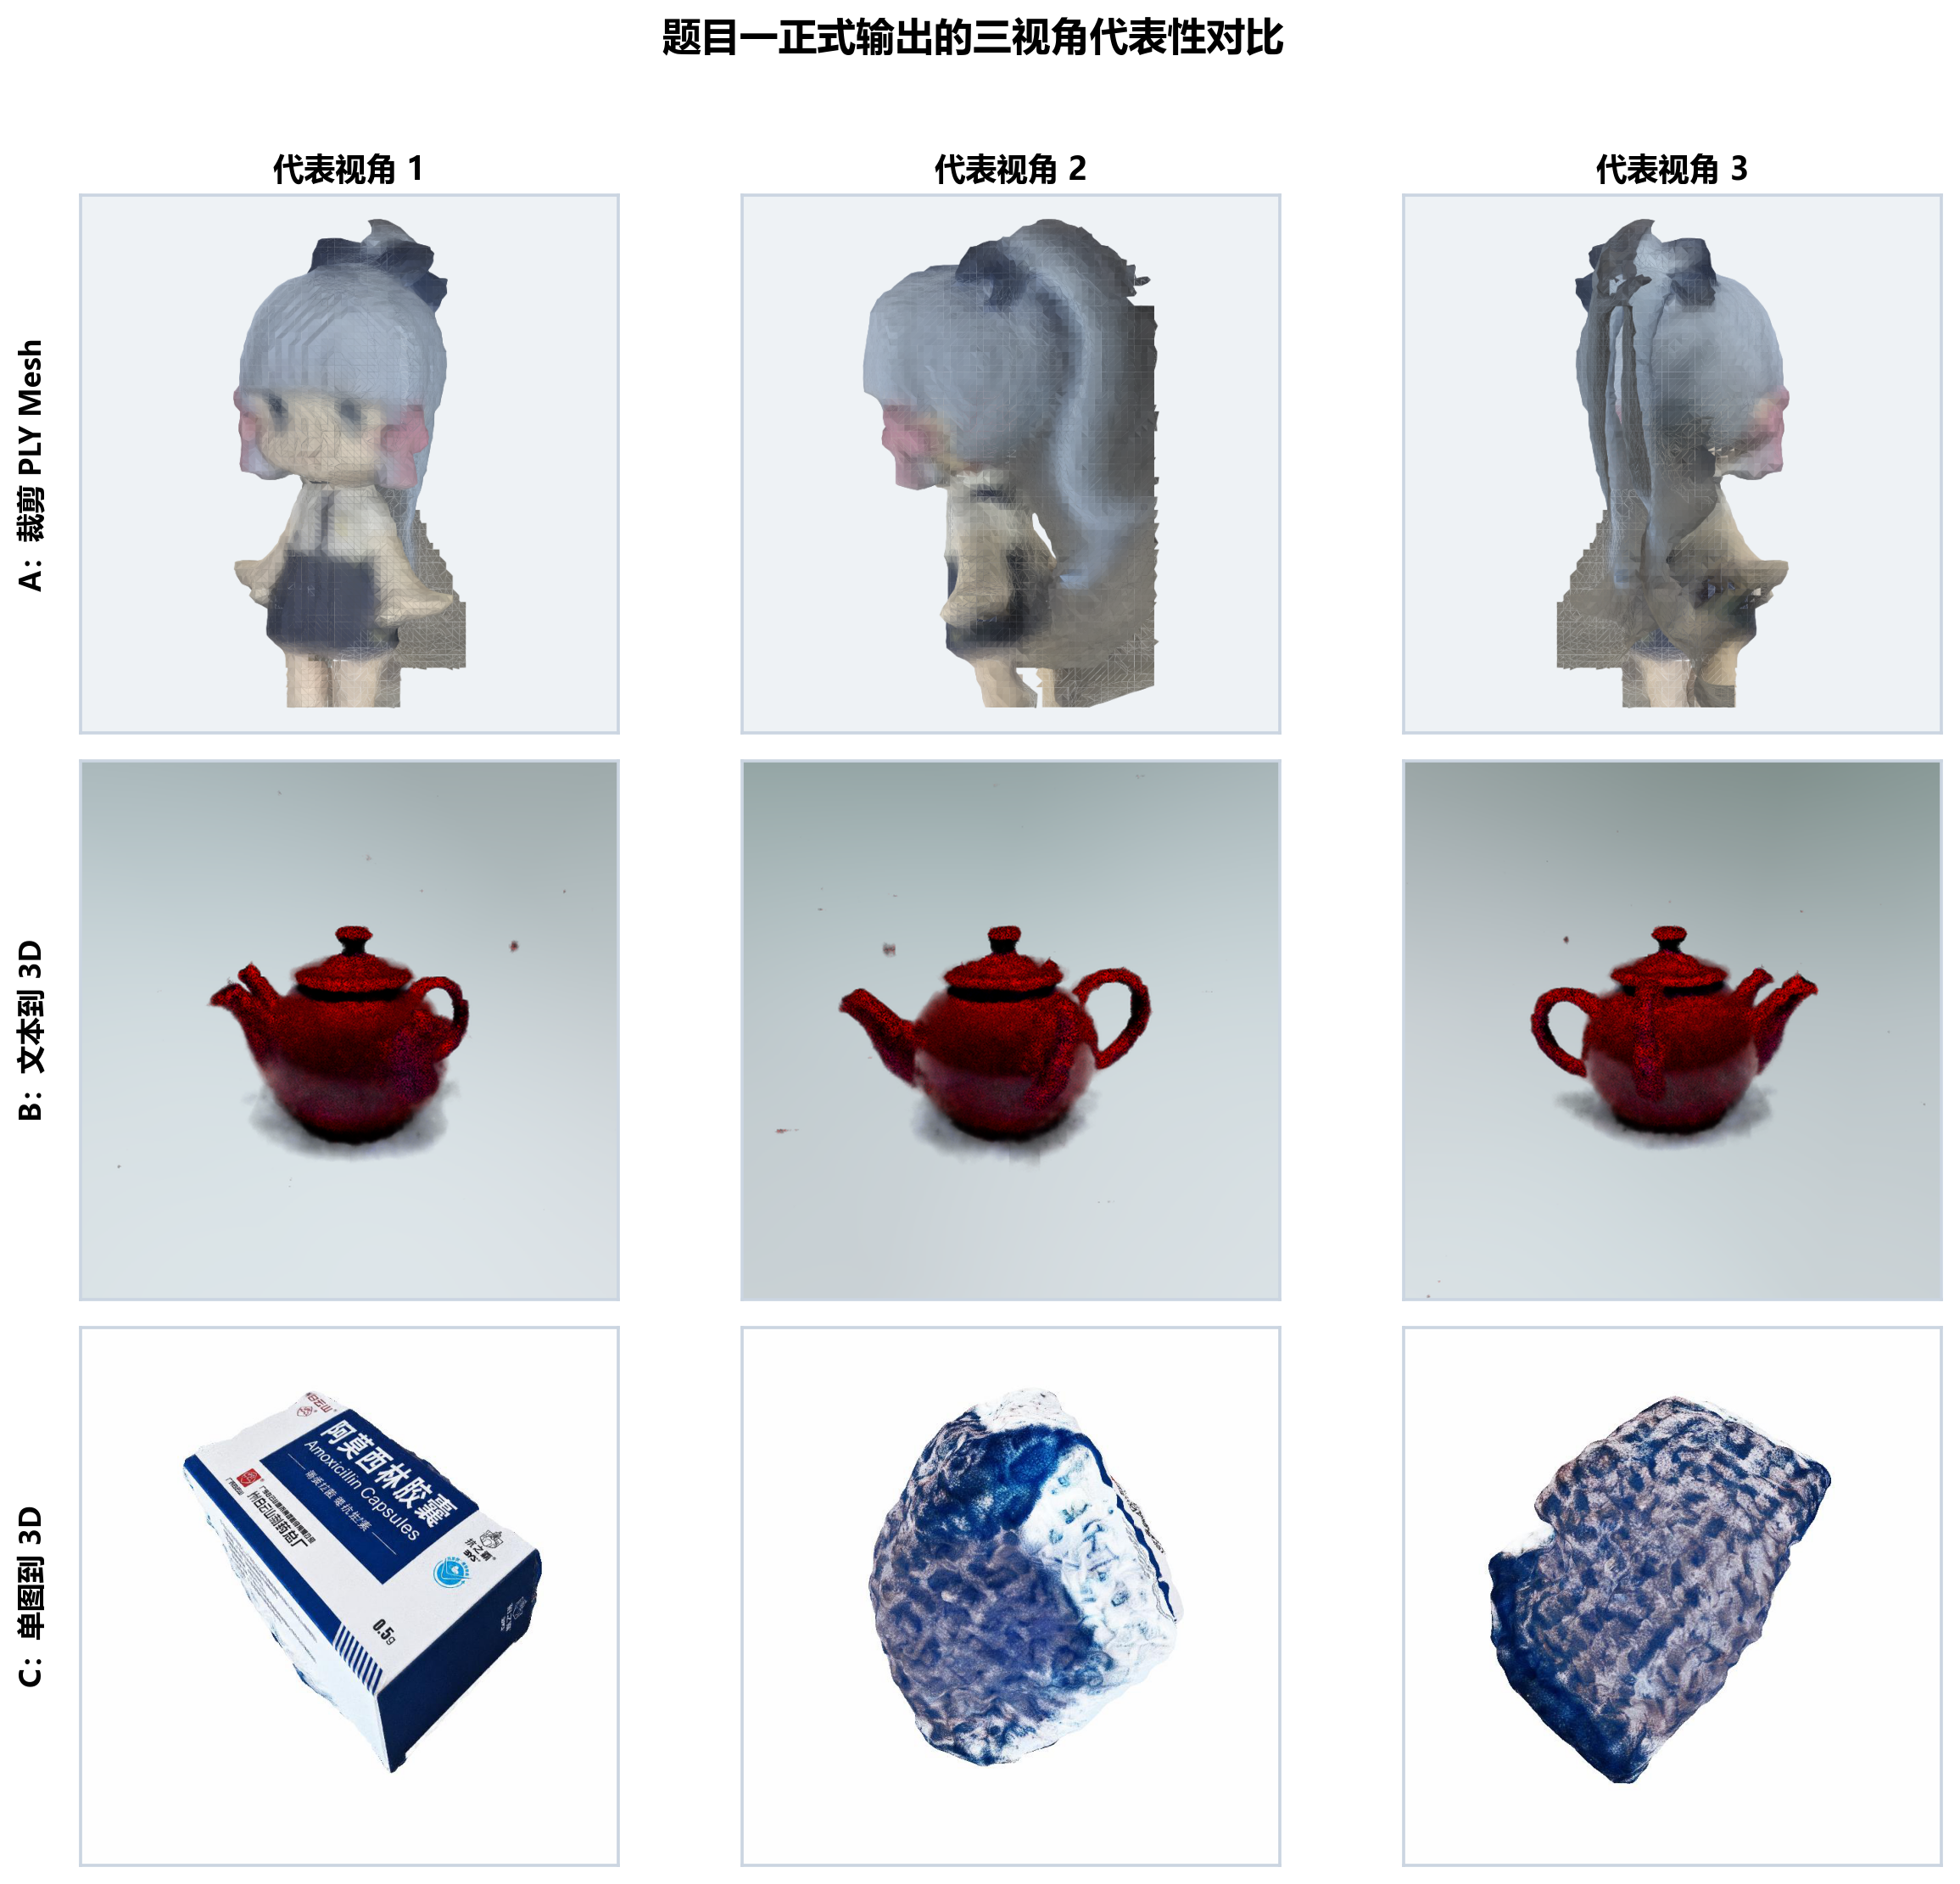
\includegraphics[width=0.94\textwidth]{task1_method_triviews.png}
  \caption{题目一三种 3D 构建方法的代表性三视图。每行对应一种方法，每列对应逐步变化的观察视角。
  上：从 2DGS 导出 PLY 中裁剪并渲染的手办 Mesh；中：文本 Prompt 驱动 DreamFusion 生成的
  红色陶瓷茶壶；下：单张药盒照片驱动 Magic123 得到的 3D 资产。}
  \label{fig:task1-triviews}
\end{figure*}

\textbf{物体 A：真实多视角重建。}
PLY Mesh 的正面仍能辨认发型、蝴蝶结、面部、服装和腿部，侧面与背面也保留了马尾的主要轮廓。
同时，网格表面比 2DGS 新视角渲染更粗糙，马尾、裙摆和腿部附近存在局部粘连，侧后方还能看到少量
TSDF 残片。手机拍摄中的视角覆盖不均、地砖反光和细小结构遮挡都会影响表面提取。多视角路线具备
较好的真实外观还原能力，导出 Mesh 的质量仍需要结合后续清理流程评估。

\textbf{物体 B：文本到 3D。}
茶壶在三个环绕视角中始终保留圆形壶身、壶盖、壶嘴和把手，类别语义和整体拓扑较稳定；这说明
SDS 优化能够从纯文本产生可用于融合渲染的完整虚拟资产。局部细节仍不够稳定：壶嘴与把手的相对
投影会随角度变化，表面还存在少量噪点，且没有真实茶壶作为几何参照。这一结果适合作为符合 Prompt
的虚拟资产，不宜用于现实对象的精确测量。

\textbf{物体 C：单图到 3D。}
药盒正面仍能保留白蓝配色、文字区域和盒装轮廓；转向侧面后，未在输入照片中出现的区域开始发生
纹理拉伸和几何鼓包；到背向视角时，规则长方体外形明显退化。该现象直接展示了单图重建的核心歧义：
可见面由照片提供强约束，不可见面只能依赖生成先验补全。受本实验 coarse/fine 优化预算限制，
Magic123 结果适合在融合场景中提供身份线索，但不适合需要精确侧后面结构的应用。

\subsubsection{几何准确度、纹理细节与计算耗时对比}

从几何准确度看，三种方法的差异主要来自输入信息量。多视角重建有真实图像和相机位姿作为约束，
物体 A 的 34 个注册视角形成了可闭合的稀疏模型，平均重投影误差为 1.192686 像素；随后 2DGS
在 30000 步达到 33.5198 dB PSNR 和 0.011289 验证 L1。图~\ref{fig:task1-triviews} 中
手办的正面、侧面和背面都能保持同一主体轮廓，这一点优于另外两种生成路线。导出 Mesh 时仍能看到
局部粘连和 TSDF 残片，说明多视角结果在真实还原上最可靠，但网格化质量还会受到拍摄覆盖、反光和
表面细节尺度的影响。文本生成的物体 B 没有真实对象作为几何目标，它得到的是符合 Prompt 的类别
形状：壶身、壶盖、壶嘴和把手在环绕视图中基本稳定，局部比例和连接处则更依赖扩散先验。单图生成
的物体 C 介于两者之间，正面由照片直接约束，侧面和背面需要推断；三视图中药盒背向视角的形变最
明显，也最能体现单图输入的几何不确定性。

纹理细节方面，多视角重建保留了实拍手办的发色、服装颜色和整体材质关系，细小边缘处会因为 Mesh
提取而变得粗糙。文本生成路线的纹理受 Prompt 控制，红色陶瓷材质整体一致，适合作为风格明确的
虚拟道具；它无法保证与某个现实茶壶完全对应。单图生成路线在药盒正面表现最好，文字区域、蓝白配色
和盒面分区都能保留下来；转到侧后方后，纹理开始拉伸并出现补全痕迹。由此看，单图方法适合保存
可见面的身份特征，完整纹理一致性仍弱于多视角实拍。

计算耗时与输入成本也需要分开看。图~\ref{fig:fusion-runtime} 和表~\ref{tab:task1-runtime}
显示，物体 A 的 COLMAP 后 2DGS 用时 4855.77 s，约 1.35 h；这还不包含手机环绕拍摄、筛图和
位姿检查的人力时间。物体 B 的 DreamFusion 训练与 OBJ 导出合计 3659.68 s，输入只需要一条文本，
是三种物体生成路线中前期准备最轻的一种。物体 C 的 Magic123 coarse 与 fine 合计 33039.31 s，
约 9.18 h，是本实验中最慢的物体生成流程；它需要同时利用二维扩散先验和新视角先验，且本机预算
已经低于论文推荐的完整迭代数。综合三视图和耗时曲线，三种路线的选择取决于任务目标：需要真实对象
还原时优先多视角重建，需要快速补充语义资产时优先文本生成，只有单张照片且希望保留对象正面特征时
可以采用单图生成。仅看一张正面预览会高估生成式 3D 的几何质量，环绕视图更能反映最终融合时的可用性。

\begin{figure*}[t]
  \centering
  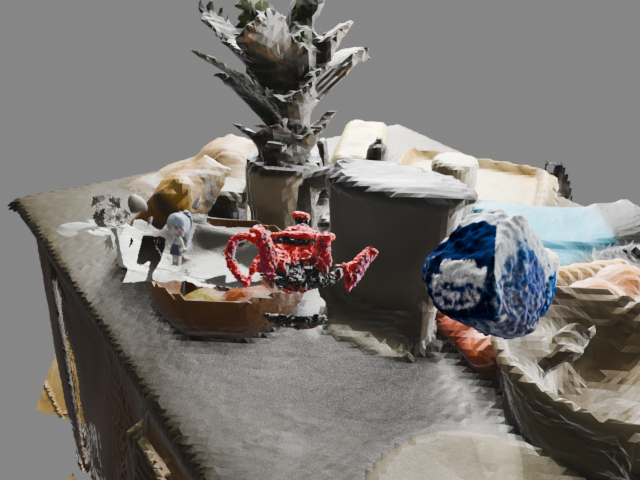
\includegraphics[width=0.49\textwidth]{fusion_walkthrough_preview.png}
  \hfill
  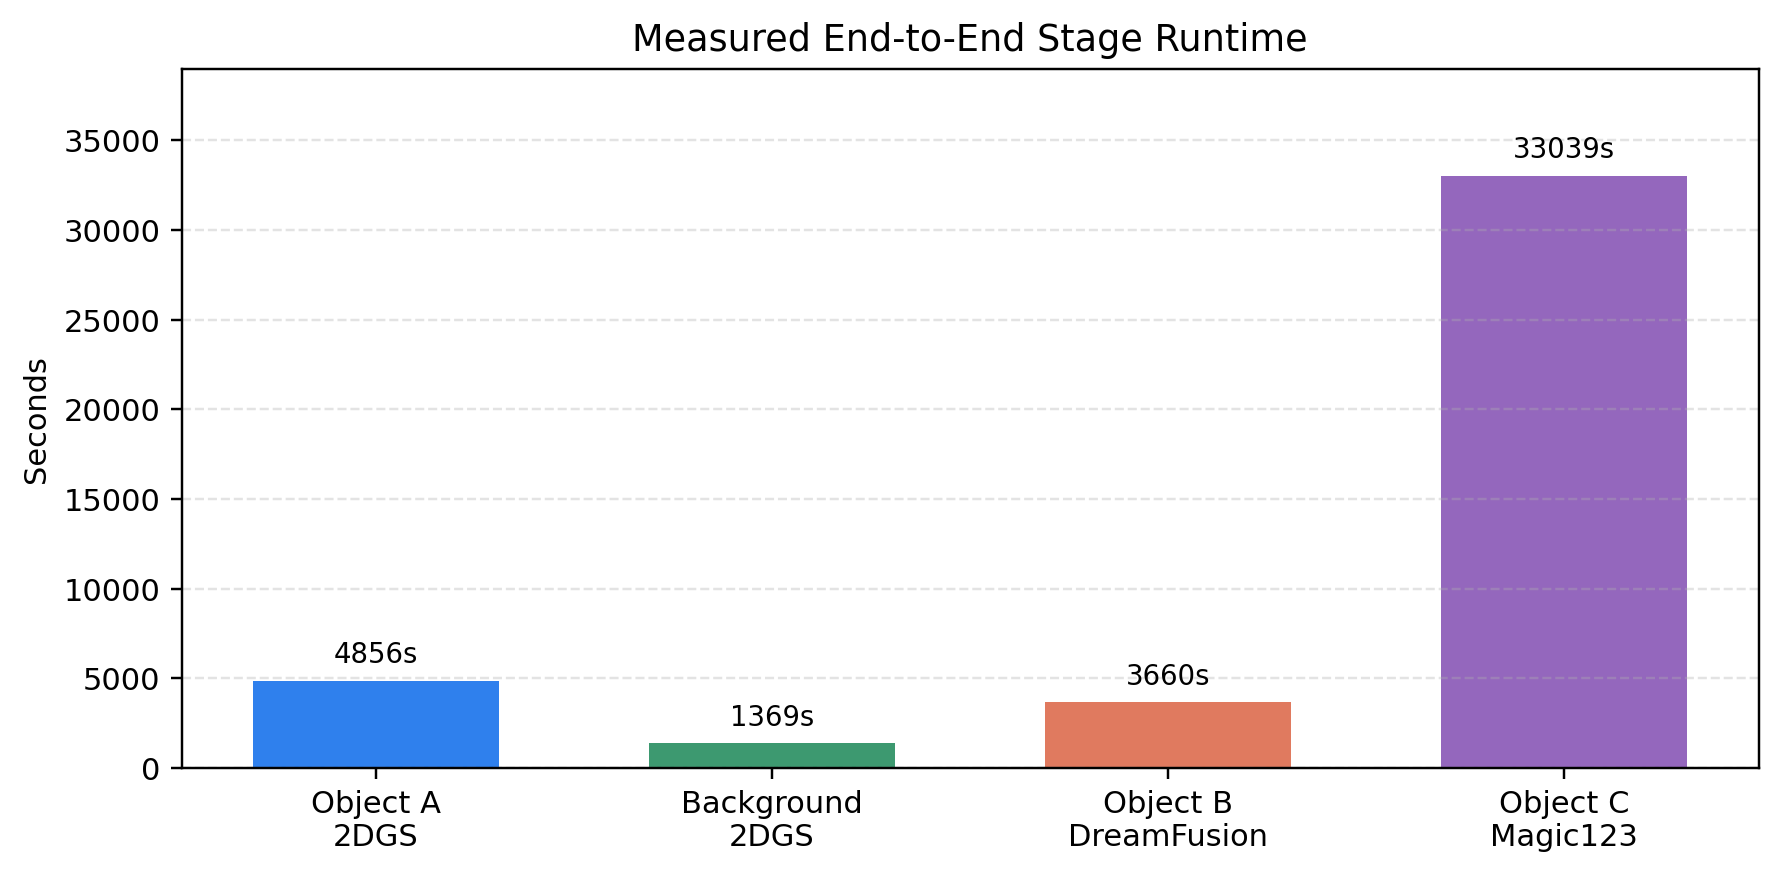
\includegraphics[width=0.49\textwidth]{runtime_comparison.png}
  \caption{左：最终融合漫游视频的代表帧。右：题目一各主要阶段的端到端耗时。}
  \label{fig:fusion-runtime}
\end{figure*}

\begin{table}[H]
\centering
\caption{题目一正式阶段耗时。}
\label{tab:task1-runtime}
\resizebox{\columnwidth}{!}{
\begin{tabular}{lrr}
\toprule
阶段 & 秒 & 约合时间 \\
\midrule
物体 A：COLMAP 后 2DGS & 4855.77 & 1.35 h \\
背景：\code{counter} 2DGS & 1368.52 & 0.38 h \\
物体 B：DreamFusion 训练 & 3624.22 & 1.01 h \\
物体 B：OBJ 导出 & 35.46 & 0.01 h \\
物体 C：Magic123 coarse & 29639.49 & 8.23 h \\
物体 C：Magic123 fine & 3399.82 & 0.94 h \\
融合视频渲染 & 5599.89 & 1.56 h \\
\bottomrule
\end{tabular}}
\end{table}

\begin{table*}[t]
\centering
\caption{三种 3D 资产构建路线的对比。}
\label{tab:task1-analysis}
\small
\begin{tabularx}{0.98\textwidth}{p{2.1cm}Y Y Y Y}
\toprule
路线 & 几何准确度 & 纹理细节 & 计算耗时与输入成本 & 适用边界 \\
\midrule
真实多视角重建 &
观测覆盖充分时最可靠；可用 COLMAP 重投影误差与 2DGS 验证指标量化 &
能保留实拍细节，但弱纹理、反光和遮挡仍会降低稳定性 &
需要环绕拍摄和位姿恢复；本实验 2DGS 训练 4855.77 s &
适合能够重新拍摄、重视真实几何的对象 \\
文本到 3D &
可得到清晰类别轮廓，但局部比例与细节受扩散先验影响，缺少真实几何监督 &
外观可由 Prompt 控制，但不保证对应现实中的某个具体物体 &
输入成本最低，仅需文本；本实验训练与导出合计 3659.68 s &
适合快速生成虚拟装饰物或原型资产 \\
单图到 3D &
正面由实拍图约束，侧后面依赖新视角先验补全，不可见区域存在歧义 &
正面纹理保持较好，侧后纹理的真实性较弱 &
采集简单但优化最慢；本实验 coarse + fine 合计 33039.31 s &
适合只有单张图、又希望保留对象身份线索的场景 \\
\bottomrule
\end{tabularx}
\end{table*}

综合来看，三条路线各有适用范围。多视角重建的输入成本最高，但可解释性也最强；文本到 3D
适合低成本资产扩展；单图到 3D 位于二者之间。统一为 Mesh 后，
Blender 能直接处理尺度、遮挡和相机运动，但代价是无法继续享受 2DGS 原生实时渲染的全部优势。

\clearpage
\section{题目二：LeRobot ACT 跨环境泛化}

\subsection{任务定义、数据规模与评估边界}

题目二要求在 CALVIN 数据集上比较两个 ACT 策略：基线仅使用环境 B 训练；联合模型使用环境
A、B、C 混合训练。二者必须采用相同网络结构和超参数，随后在训练阶段完全不可见的环境 D 上进行
zero-shot 评估。本实验将 D 环境 zero-shot 分成两个层级：第一层在官方 D validation 抽样帧上
计算 first-action MAE 与 chunk-action MAE；第二层把两个最佳 checkpoint 包装成 CALVIN
\code{reset}/\code{step} 策略，在 \code{calvin\_scene\_D} simulator 中执行闭环 rollout。
rollout 使用官方任务 oracle、validation language annotations、3 条自动生成的五任务序列，
每个子任务最多执行 360 步。该设置能够验证模型是否能部署到未见环境 D，但规模仍小于 CALVIN
完整长时评测协议。

官方 CALVIN 元数据给出的训练帧范围如表~\ref{tab:calvin-ranges}。完整 A+B+C 压缩包约
517 GB，D 环境压缩包约 166 GB。为在本机完成可复现实验，项目实现 HTTP Range 下载器：
从官方压缩包中均匀抽取连续窗口、验证 CRC，并保持原始目录结构，不需要下载完整归档。

\begin{table}[H]
\centering
\caption{CALVIN 官方训练帧范围。}
\label{tab:calvin-ranges}
\begin{tabular}{lr}
\toprule
环境 & 官方闭区间 \\
\midrule
B & 0--598909 \\
C & 598910--1191338 \\
A & 1191339--1795044 \\
\bottomrule
\end{tabular}
\end{table}

\begin{table}[H]
\centering
\caption{题目二资源约束下的正式子集协议。}
\label{tab:task2-subset}
\resizebox{\columnwidth}{!}{
\begin{tabular}{lccc}
\toprule
用途 & 选取帧数 & 本地数据量 & 处理后样本数 \\
\midrule
A+B+C 训练源数据 & 2304 & 634.01 MiB & 691 训练 / 77 验证 \\
B-only 训练源数据 & 768 & 包含于上行 & 230 训练 / 26 验证 \\
D 环境 zero-shot 评估 & 768 & 212.78 MiB & 768 离线帧；3 条 rollout 序列 \\
\bottomrule
\end{tabular}}
\end{table}

本地实际使用的 CALVIN 帧数据合计 887929630 bytes，约 846.8 MiB，其中 A+B+C 训练源数据
约 634.01 MiB，D 环境离线评估数据约 212.78 MiB。另有约 287.97 MiB 的
\code{.cache} 索引文件，用于定位远程 ZIP 中的条目。训练数据使用 stride 3 与 90/10
训练验证划分。B-only 与 A+B+C 模型的样本数量不同，联合训练模型能够接触三种场景的视觉多样性；
二者的网络、优化器、步数和评估脚本完全一致，因此差异主要来自训练环境分布变化。

\subsection{ACT 策略与动作分块机制}

ACT（Action Chunking with Transformers）根据当前图像和机器人状态一次预测未来 $K$ 步动作块：
\begin{equation}
  \hat{\mathbf{a}}_{t:t+K-1}
  = \pi_{\theta}(\mathbf{o}_{t}, \mathbf{s}_{t}).
\end{equation}
本实验使用 LeRobot v0.5.1 中的 \code{ACTPolicy}，输入为 $128\times128$ RGB 图像和
15 维状态，输出为 7 维动作，动作块长度 $K=20$。模型包含 ResNet-18 视觉骨干、Transformer
编码器与解码器，以及条件 VAE 潜变量。训练目标可概括为
\begin{equation}
  \mathcal{L}_{\text{ACT}}
  = \mathcal{L}_{1}(\hat{\mathbf{a}},\mathbf{a})
  + \lambda_{\text{KL}}\mathcal{L}_{\text{KL}},
  \qquad \lambda_{\text{KL}}=10.
\end{equation}

动作分块对视觉偏移具有两面性。一方面，一次预测一段动作可以减少单帧噪声引起的控制抖动，并让
轨迹更连贯；另一方面，若视觉表征在新环境中发生系统性偏差，较长 horizon 也会累积不确定性。
因此，本实验同时报告 first-action MAE 与 chunk-action MAE：前者反映立即决策质量，后者更严格
地反映整段预测的鲁棒性。

\subsection{题目二实验设置}

\begin{table*}[t]
\centering
\caption{题目二 ACT 正式实验超参数。两个训练条件完全一致，仅训练环境不同。}
\label{tab:task2-hyper}
\small
\begin{tabularx}{0.98\textwidth}{p{2.55cm}p{2.05cm}p{2.7cm}p{2.05cm}Y}
\toprule
项目 & 取值 & 项目 & 取值 & 说明 \\
\midrule
视觉骨干 & ResNet-18 & 图像尺寸 & $128\times128$ & 不加载预训练 backbone 权重 \\
Transformer 维度 & 256 & attention heads & 8 & feedforward 维度 1024 \\
编码器 / 解码器层数 & 3 / 1 & 动作块长度 & 20 & 推理时输出 20 步动作 \\
状态 / 动作维度 & 15 / 7 & VAE latent 维度 & 32 & VAE 编码器 2 层，KL 权重 10 \\
优化器 & AdamW & 学习率 & $1\times10^{-5}$ & backbone 使用相同学习率 \\
权重衰减 & $1\times10^{-4}$ & batch size & 4 & AMP 开启，梯度裁剪范数 10 \\
训练步数 & 5000 & 验证间隔 & 250 & 每次验证 30 batches \\
设备 & RTX 4060 Ti & 显存 & 8 GB & Windows 本地 CUDA 环境 \\
\bottomrule
\end{tabularx}
\end{table*}

\subsection{收敛情况、动作误差与 simulator rollout}

\begin{figure*}[t]
  \centering
  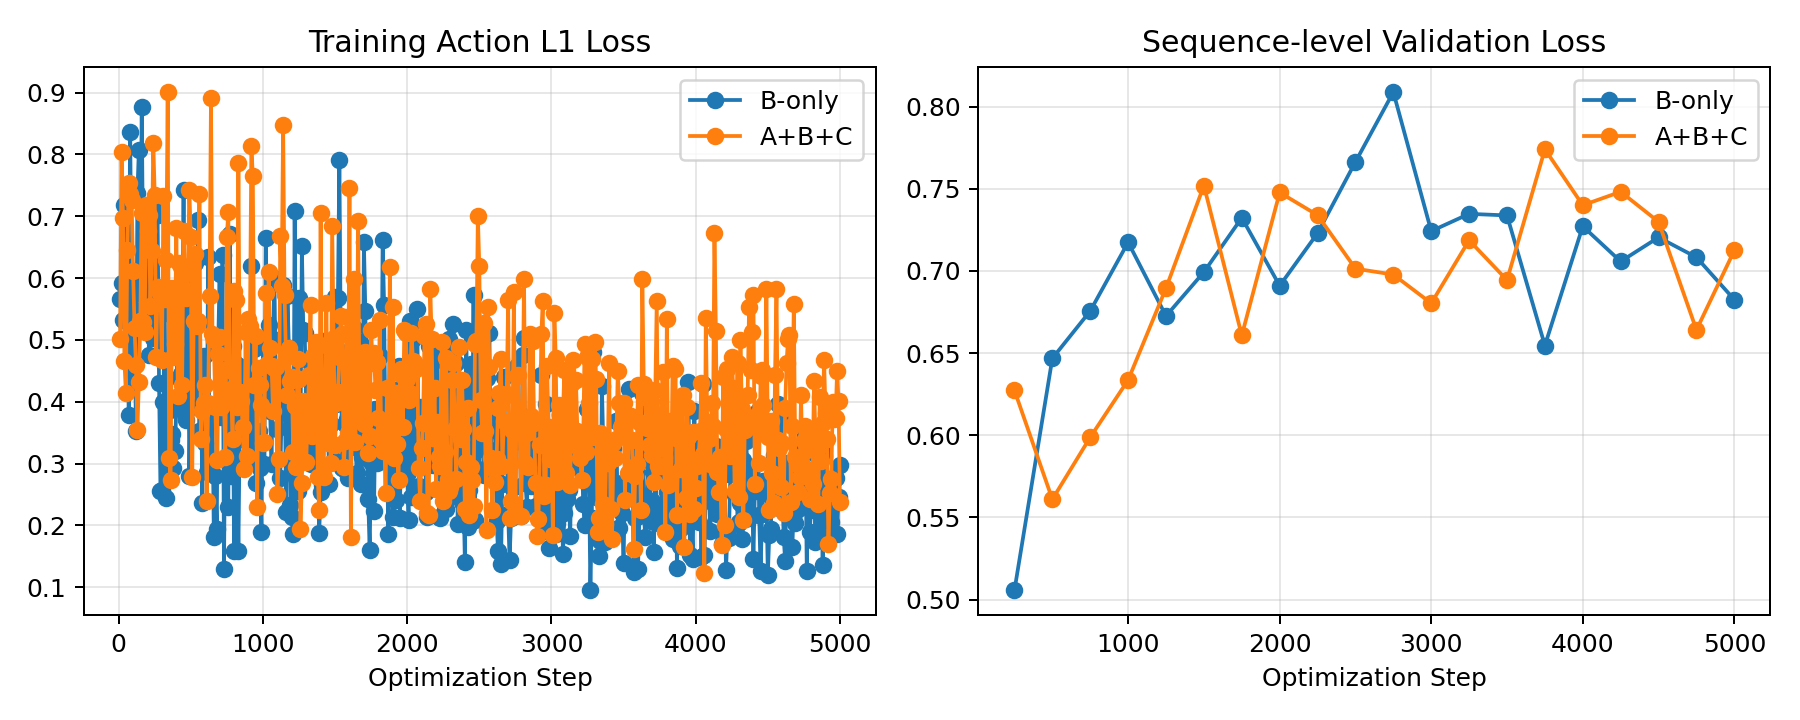
\includegraphics[width=0.96\textwidth]{formal_training_curves.png}
  \caption{由 SwanLab 记录指标导出的 ACT 训练 Action L1 与 held-out 验证曲线。
  A+B+C 联合模型面对更复杂的视觉分布，因此验证损失更高；两个条件均呈下降趋势。}
  \label{fig:act-curves}
\end{figure*}

\begin{table}[H]
\centering
\caption{ACT 正式实验结果。MAE 越低越好。}
\label{tab:act-results}
\resizebox{\columnwidth}{!}{
\begin{tabular}{lrrr}
\toprule
训练环境 & 验证 L1 & D first-action MAE & D chunk MAE \\
\midrule
B-only & 0.324629 & 0.226251 & 0.259475 \\
A+B+C & 0.386954 & \textbf{0.187712} & \textbf{0.229145} \\
\bottomrule
\end{tabular}}
\end{table}

\begin{figure}[H]
  \centering
  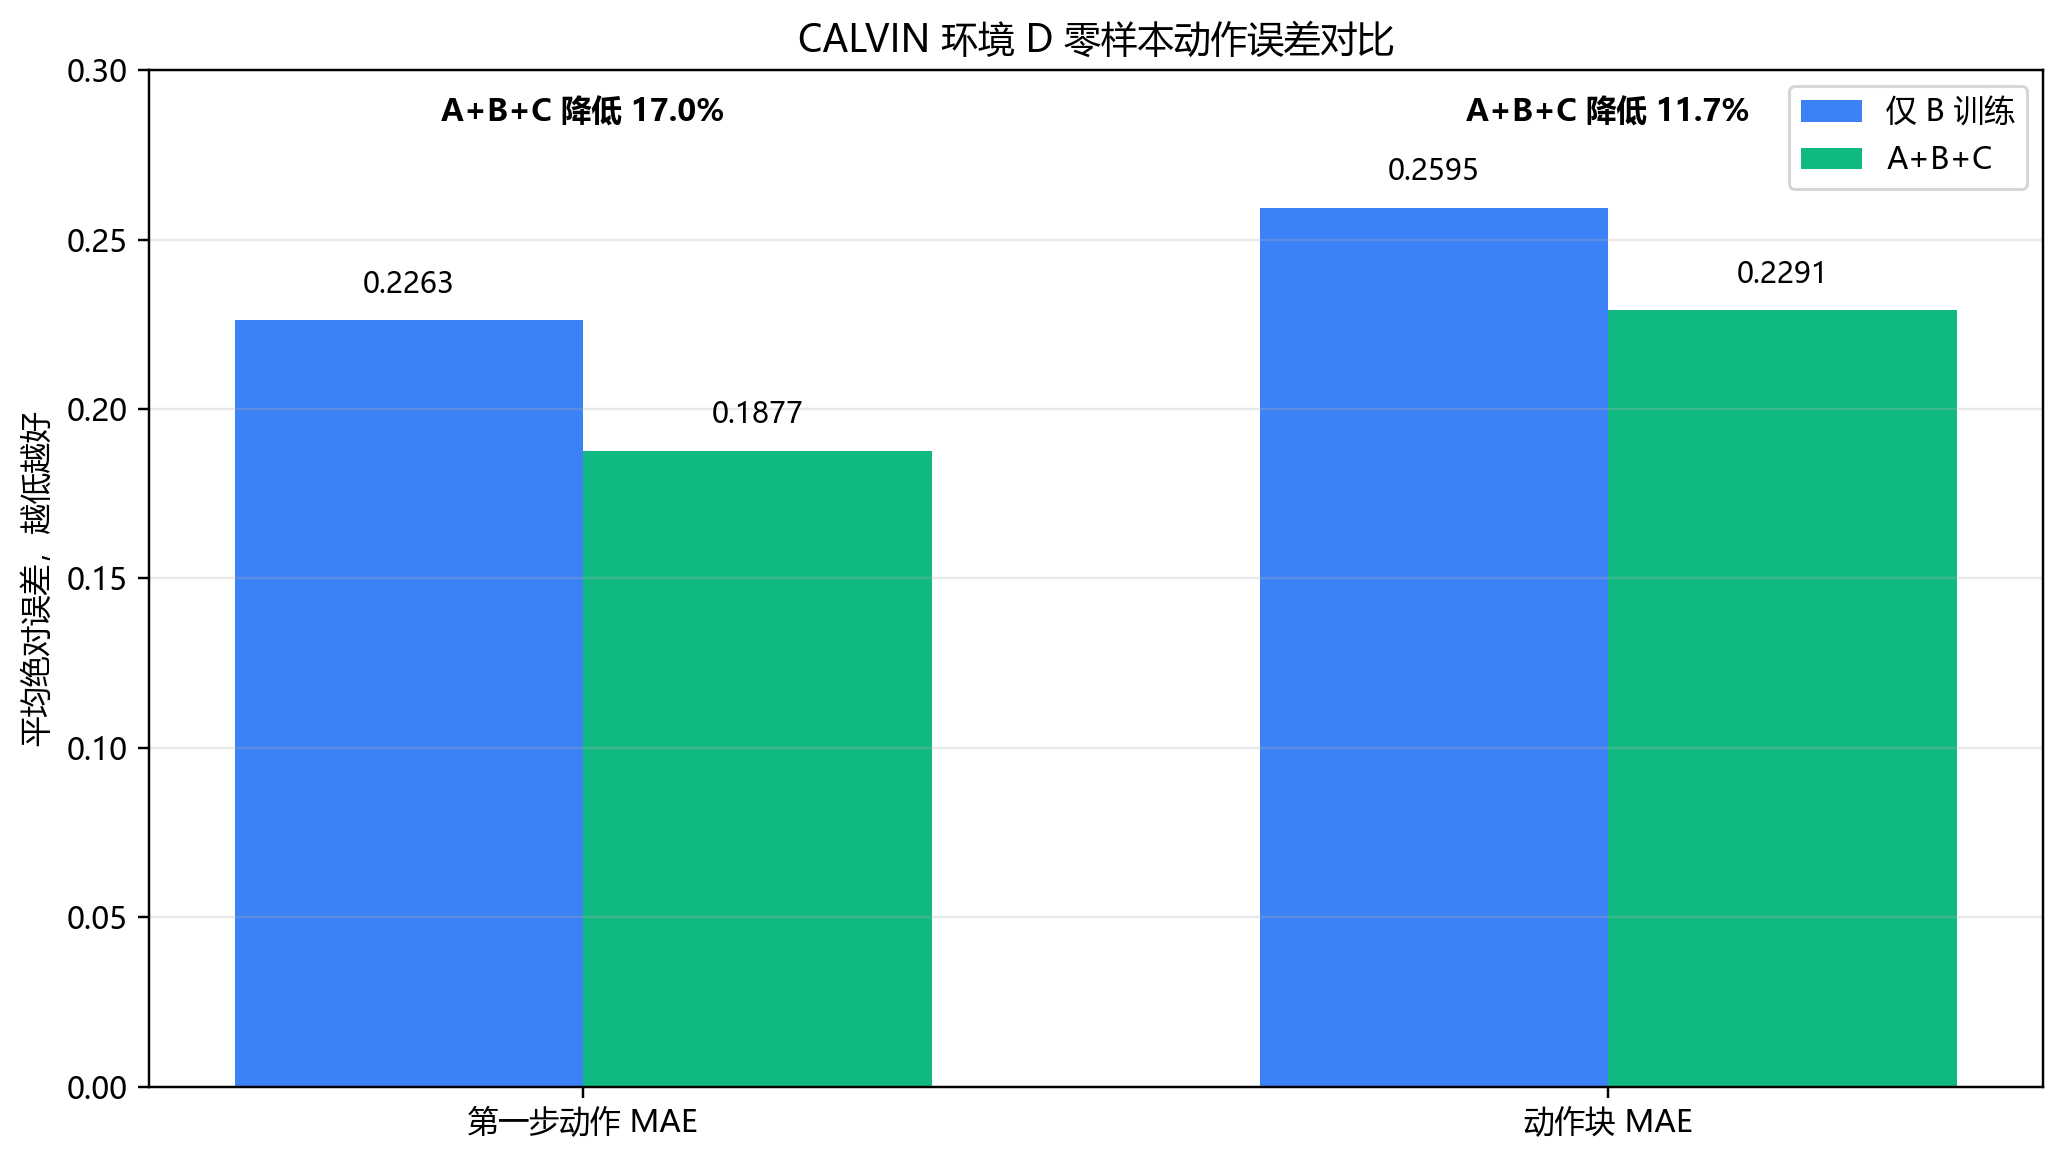
\includegraphics[width=0.98\columnwidth]{task2_zero_shot_grouped.png}
  \caption{环境 D 抽样帧上的离线 zero-shot 动作误差。与 B-only 相比，A+B+C 联合训练使 first-action
  MAE 下降 17.0\%，chunk-action MAE 下降 11.7\%。}
  \label{fig:act-zeroshot}
\end{figure}

\begin{table*}[t]
\centering
\caption{环境 D simulator rollout 结果。每个模型评估 3 条五任务序列，每个子任务最多 360 步。}
\label{tab:rollout-results}
\small
\begin{tabularx}{0.98\textwidth}{p{2.0cm}p{1.45cm}p{2.3cm}p{1.2cm}p{1.2cm}p{1.2cm}p{1.2cm}p{1.2cm}Y}
\toprule
训练环境 & 序列数 & 平均完成子任务数 & SR@1 & SR@2 & SR@3 & SR@4 & SR@5 & 记录位置 \\
\midrule
B-only & 3 & 0.0 / 5 & 0.0 & 0.0 & 0.0 & 0.0 & 0.0 &
对应 rollout 输出目录中的 metrics JSON \\
A+B+C & 3 & 0.0 / 5 & 0.0 & 0.0 & 0.0 & 0.0 & 0.0 &
对应 rollout 输出目录中的 metrics JSON \\
\bottomrule
\end{tabularx}
\end{table*}

\subsection{现象分析：视觉偏移与动作分块}

表~\ref{tab:act-results} 中最值得注意的现象是：A+B+C 模型的 held-out 验证 L1 为
0.386954，高于 B-only 的 0.324629，但它在未见环境 D 上的误差更低。B-only 验证集仍来自
单一环境 B，视觉分布窄，模型更容易拟合；联合模型需要同时处理 A、B、C
中的外观变化，优化问题更难，因此同分布验证误差较高。然而，这种训练阶段的视觉多样性减少了
模型对环境 B 背景细节的依赖，使它迁移到 D 时更加稳健。

first-action MAE 的改善幅度为 17.0\%，而 chunk-action MAE 的改善幅度为 11.7\%。后者较小，
说明在视觉分布偏移下，长 horizon 预测仍会累积不确定性。chunk MAE 同样下降，表明多环境训练
同时改善了立即决策和整段 20 步预测。动作分块为短期轨迹提供时间一致性，多环境视觉训练则降低了
错误视觉线索对整个动作块的传播。

表~\ref{tab:rollout-results} 给出的 simulator rollout 结果更严格。两个模型都能加载到
CALVIN D 场景中并完成 \code{reset}/\code{step} 闭环调用，说明 zero-shot 部署链路已经打通；
但 3 条五任务序列的 SR@1--SR@5 均为 0。这个结果与离线 action-error 的改善并不矛盾。
离线 MAE 衡量的是给定一帧观测时预测动作与专家动作的平均距离，数值下降说明模型在 D 环境的局部
动作回归更接近数据分布。CALVIN rollout 成功率衡量的是长时闭环任务：策略必须根据当前图像、状态
和任务序列连续推动环境变化，任一早期子任务失败都会使后续任务无法继续计入。

本实验使用的 ACT 输入为图像和机器人状态，没有显式语言指令输入；rollout adapter 会接收官方
validation annotations，但模型内部并不使用语言条件。因此，模型更接近一个从观测到动作块的
模仿策略，尚未具备完整语言条件长时任务策略的输入结构。动作分块在这种闭环评估中也会放大偏差：一旦某次
观测产生了偏离目标的 20 步动作块，错误会在一段时间内连续作用到环境，随后再用已经偏移的状态
预测下一个动作块。多环境训练能降低视觉偏移造成的局部动作误差，但在小规模数据、无语言条件和
长时任务链条同时存在时，还不足以把这种局部改善转化为非零成功率。

\subsection{题目二局限性}

题目二使用官方 CALVIN 帧的均匀抽样子集，覆盖 846.8 MiB 本地帧数据，未使用完整的
517 GB / 166 GB 数据归档。simulator rollout 已经完成，但只评估了 3 条五任务序列，远小于
完整 CALVIN 长时 benchmark 的规模；因此成功率只能作为小规模部署验证结果，而不能代表充分训练
后的最终任务能力。离线 action-error 可以衡量模型输出动作与数据集中专家动作的接近程度，也能
反映一定的跨环境泛化差异；rollout success 则进一步考察闭环执行、误差累积和任务链条恢复能力。
因此，本实验结论限定在报告所述资源约束协议内：多环境联合训练提升了未见环境 D 的离线动作泛化，
但在当前小规模 simulator rollout 中尚未产生可统计的成功子任务。

\clearpage
\onecolumn
\section{复现、SwanLab 与交付物}

\subsection{SwanLab 记录}

\begin{table}[H]
\centering
\caption{实验记录与公开链接。}
\label{tab:swanlab}
\small
\begin{tabularx}{0.98\textwidth}{p{3.8cm}Y}
\toprule
项目 & 记录方式或链接 \\
\midrule
题目一 2DGS / DreamFusion / Magic123 &
SwanLab local runs；报告图由记录标量导出。本地查看命令：
\code{swanlab watch hw3/task1/swanlog} \\
题目二项目页 &
\url{https://swanlab.cn/@Linkukai/hw3-calvin-act} \\
题目二 B-only 训练 &
\url{https://swanlab.cn/@Linkukai/hw3-calvin-act/runs/y34dmlyk6ol06me1f1ig0} \\
题目二 A+B+C 训练 &
\url{https://swanlab.cn/@Linkukai/hw3-calvin-act/runs/t3kfag5dsiipp3wwxy4te} \\
题目二 B-only $\rightarrow$ D 评估 &
\url{https://swanlab.cn/@Linkukai/hw3-calvin-act/runs/b1hdsdo4vgrodwkk3syr7} \\
题目二 A+B+C $\rightarrow$ D 评估 &
\url{https://swanlab.cn/@Linkukai/hw3-calvin-act/runs/5ooypxeqhgp4xja928tpk} \\
题目二 B-only $\rightarrow$ D rollout &
\url{https://swanlab.cn/@Linkukai/hw3-calvin-act/runs/kcbgr0rmn3jokevjmxlyj} \\
题目二 A+B+C $\rightarrow$ D rollout &
\url{https://swanlab.cn/@Linkukai/hw3-calvin-act/runs/mqrmkx48ojvthl5gm0u2y} \\
\bottomrule
\end{tabularx}
\end{table}

\subsection{关键复现入口}

题目一与题目二均整理在统一仓库 \url{https://github.com/Loong-C/FDU-Computer-Vision} 的
\code{main/hw3} 路径下，分别位于 \code{hw3/task1} 与 \code{hw3/task2}。两个目录均提供
README、环境依赖、数据准备说明、训练命令与测试命令。下面仅列出主入口；完整命令、兼容性说明与
缓存设置见对应目录 README。

\begin{lstlisting}[language=bash,caption={题目一主要复现入口。}]
# 物体 A 与背景：COLMAP + 2DGS
bash scripts/prepare_colmap_object_a.sh --force
bash scripts/train_2dgs_object_a.sh
bash scripts/train_2dgs_background.sh

# 文本到 3D 与单图到 3D
MODE=full bash scripts/generate_text3d_object_b.sh
MODE=full STAGE=coarse bash scripts/generate_image3d_object_c.sh
MODE=full STAGE=fine bash scripts/generate_image3d_object_c.sh

# 统一 Mesh 后融合渲染
MODE=formal bash scripts/render_fusion_tracked.sh
\end{lstlisting}

\begin{lstlisting}[language={},caption={题目二主要复现入口（PowerShell）。}]
.\scripts\bootstrap.ps1
.\scripts\run_partial_formal.ps1
.\scripts\bootstrap.ps1 -WithCalvinRollout
.\scripts\run_zero_shot_d_rollout.ps1 `
  -MaxSequences 3 `
  -EpisodeLength 360 `
  -Device cuda
\end{lstlisting}

\subsection{公开下载与校验}

\begin{table}[H]
\centering
\caption{公开交付物。题目一与题目二均使用 FDU 仓库 GitHub Release，Google Drive 作为镜像。}
\label{tab:deliverables}
\small
\begin{tabularx}{0.98\textwidth}{p{3.2cm}p{2.4cm}Y}
\toprule
交付物 & 大小 & 下载地址或 SHA256 \\
\midrule
题目一最佳资产包 &
274591842 bytes &
\url{https://github.com/Loong-C/FDU-Computer-Vision/releases/download/hw3-task1-weights/cv-hw3-task1-best-weights.tar.gz} \\
题目一漫游视频 &
1545398 bytes &
\url{https://github.com/Loong-C/FDU-Computer-Vision/releases/download/hw3-task1-weights/task1-walkthrough.mp4} \\
题目一资产包 SHA256 &
-- &
\code{4667c06b2e05b4a345f99ae5ee4c2875caaad2f995ad77c6ea813814046ccaec} \\
题目二 B-only 最佳权重 &
196370804 bytes &
\href{\tasktwobweights}{GitHub Release 下载}；
\code{58afae052ef2ce029f92c9258e1b5012a9c44fac5753c1c8330b7d196a976131} \\
题目二 A+B+C 最佳权重 &
196370804 bytes &
\href{\tasktwoabcweights}{GitHub Release 下载}；
\code{1b1f182e61026929f0a5ffdc5ee096d15e4771febd111d9efe3d88bc4a9adcff} \\
题目二权重 Release &
-- &
\href{\tasktworelease}{FDU GitHub Release 页面} \\
Google Drive 镜像目录 &
-- &
\href{\clouddrive}{Google Drive 镜像文件夹} \\
\bottomrule
\end{tabularx}
\end{table}

\clearpage
\section{结论}

题目一完成了从真实采集、文本生成、单图生成到真实场景融合的完整链路。实验说明，多视角重建、
文本到 3D 和单图到 3D 各自适合不同的信息条件；当原生表示不一致时，将资产转换为 Mesh 再进入
Blender 是一种工程上直接、稳定且便于控制的统一方案。题目二完成了相同 ACT 架构下的训练分布
对照：A+B+C 联合训练虽然增加了拟合难度，却降低了未见环境 D 上的离线动作误差。进一步的
CALVIN D simulator rollout 表明，两个模型都可以在未见 D 场景中完成闭环部署，但当前 3 条
五任务序列的成功率仍为 0。该现象支持视觉多样性训练有助于局部动作泛化，同时也说明动作分块、
语言条件缺失和长时误差累积仍是闭环成功率的主要限制。

\begin{thebibliography}{9}
\small
\bibitem{2dgs}
B. Huang et al.
\newblock 2D Gaussian Splatting for Geometrically Accurate Radiance Fields.
\newblock SIGGRAPH 2024. \url{https://arxiv.org/abs/2403.17888}

\bibitem{dreamfusion}
B. Poole et al.
\newblock DreamFusion: Text-to-3D using 2D Diffusion.
\newblock ICLR 2023. \url{https://arxiv.org/abs/2209.14988}

\bibitem{magic123}
G. Qian et al.
\newblock Magic123: One Image to High-Quality 3D Object Generation Using Both 2D and 3D Diffusion Priors.
\newblock ICLR 2024. \url{https://arxiv.org/abs/2306.17843}

\bibitem{mipnerf360}
J. T. Barron et al.
\newblock Mip-NeRF 360: Unbounded Anti-Aliased Neural Radiance Fields.
\newblock CVPR 2022. \url{https://arxiv.org/abs/2111.12077}

\bibitem{calvin}
O. Mees et al.
\newblock CALVIN: A Benchmark for Language-Conditioned Policy Learning for Long-Horizon Robot Manipulation Tasks.
\newblock IEEE RA-L 2022. \url{https://arxiv.org/abs/2112.03227}

\bibitem{act}
T. Z. Zhao et al.
\newblock Learning Fine-Grained Bimanual Manipulation with Low-Cost Hardware.
\newblock RSS 2023. \url{https://arxiv.org/abs/2304.13705}

\bibitem{lerobot}
Hugging Face.
\newblock LeRobot: State-of-the-art Machine Learning for Real-World Robotics in Pytorch.
\newblock \url{https://github.com/huggingface/lerobot}
\end{thebibliography}

\end{document}
